\chapter{Hypothesis Testing}

\nl \textbf{Motivational example:}

\nl I claim that I am a 75\% free-throw shooter. You need to verify, and make me shoot 20 free throws. \color{red}I make 8.\color{black}

\nnl You are suspicious of my claim.

\nl Is that suspicion founded?

\nl We can think of a free-throw as $\operatorname{Bern}(0.75)$.

\nl The probability of getting 8 is binomial.
    $$\P{X = 8} = \binom{20}{8} \pars{\frac{3}{4}}^8 \pars{\frac{1}{4}}^{12} = 0.00075$$

\nl This implies that if $p = \frac{3}{4}$ is true, we observed a \say{rare event.}

\nl But, another way to think about this is if $p = \frac{3}{4}$, what is the probability that I would shoot 8 or worse?

$$\P{X \leq 8} = \sum_{i=0}^8 \binom{20}{i} \pars{\frac{3}{4}}^{i} \pars{\frac{1}{4}}^{20-i} < 0.001$$

\nl The entire array, $0, 1, \dots, 8$ is less than $\over{1000}$ probability. We are \say{safe} to conclude that the true free-throw percentage is less than 75\%.

\nl This is what hypothesis testing is all about.
\begin{itemize}
    \item Assume something is true
    \item Observe and compute the probabilty of this outcome, or more extreme (rarer) events.
    \item Decide if there is evidence against your assumption.
\end{itemize}

\nl Flip-side: In chapter 8 we would have constructed a confidence interval for the true $p$.

\nl $n = 20$ is small... we need $t(\df = 19)$ distribution.

\nl A 99\% C.I. for $p$

\nl Uses $t_{0.005}(19) = 2.861 \text{ standard errors}$.
$$\phat \pm t_{0.005}\sqrt{\frac{\phat\qhat}{20}} \approx 0.4 \pm 0.256 \implies p \in (0.144, 0.656)$$

\nl \color{red} $p = \dfrac{3}{4}$ is very far outside.\color{black} \hspace{.5mm} Again, very unlikely that $p = \dfrac{3}{4}$.\\
*C.I. and the Hypothesis Test are 2-sides of the same coin.

\nnl Hypothesis Testing Vocab
\begin{enumerate}[label=\textcircled{\raisebox{-1pt}{\arabic*}}]
    \item The Hypotheses.
    \begin{itemize}
        \item \textbf{\color{neonorange}The null hypothesis} $H_0$ : Assumption of no change.
        \\ Assumed true unless \say{proven} otherwise.
        \\\example* $H_0 : p_0 = 0.75$
        \item \textbf{\color{neonorange}The alternative hypothesis} $H_a$ : The claim we aim to test.
        \\ $H_a : p < 0.75$
        \\\example*{One sided} $H_a : p < p_0$ or $H_a : p > p_0 $
        \\\example*{Two sided} $H_a : p \neq p_0$
    \end{itemize}
    \item \textbf{\color{neonorange}The decision rule}. This is the cutoff \setRed $\alpha$ \setBlack we use to accept or reject $H_a$. Usually stated beforehand.
    \item \textbf{The decision}. After a probability calculation, either
    \begin{enumerate}[label=(\roman*)]
        \item Reject the null hypothesis $H_0$ or
        \item Not enough evidence to reject $H_0$ (accept $H_a$)
    \end{enumerate}
    \item \textbf{$p$-value.} The probability of seeing as much, or more evidence for $H_a$ than we saw in the data.
    $$p = \P{X \leq 8} < 0.001$$
    *The smaller the $p$-value, the more support for $H_a$.
    \\Test Results are called \textbf{statistically significant} if $H_0$ is rejected.
\end{enumerate}

\nnl \textbf{Topic: Error Types}

\nl 2 possible decisions $\implies$ 2 possible mistakes.


  \begin{center}
    \begin{tabular}{|l|c|c|} 
         \hline
         The \say{truth} & $H_0$ & $H_a$\\
         \hline\hline
         Test Supports $H_0$ & \green{good} & \red{Type II}\\
         Test Supports $H_a$ & \red{Type I} & \green{good}\\
         \hline
    \end{tabular}
\end{center}

    %H_0  |  H_a  |  "The truth"
%H_0 Good   Type II
%H_1 Type I  Good
%^test supports

\nnl \textbf{Type I:} We reject $H_0$ when $H_0$ is the truth.\\
*This error comes from the decision rule.\\
\example* I actually am a 75\% free-throw shooter, but had a bad day.

\nl \textbf{Type II:} We accept $H_0$ when $H_a$ is the truth.

\nnl We will see that we can measure these error types in some sense, but it depends on our decision rule \setRed $\alpha$ \setBlack and the unknown, true population parameter $\theta$.
\begin{align*}
    &\P{\text{Type I error}} = \alpha.\\
    &\P{\text{Type II error}} = \beta.
\end{align*}


\example* Back to the free throws.

\nl \textit{Decision Rule:} Beforehand, you decide if I make 10 or less, you will reject $H_0 : p = 0.75$.

\nl The text calls the set of outcomes the \underline{\textbf{\color{neonorange}rejection region}} (RR). If $T \in \operatorname{RR}$ then we reject $H_0$ (support the alternative).

\nl Here, $RR = \{0,1,2,\dots,10\}$ and we can exactly calculate this:
\begin{align*}
    \alpha &= \P{\text{Type I error}}\\
    &= \P{\text{rejecting } H_0 \text{ when } H_0 \text{ is true}}\\
    &= \P{0 \leq T \leq 10 \;\text{ and }\; p = \frac34}\\
    &= \operatorname{pbinom}(10,\;20,\;0.75)\\
    &= 0.013
\end{align*}
Hence, it is very unlikely to get a Type I error.

\nl Computing Type II error probabilities requires a guess for the true $H_a$.

\begin{align*}
    \beta &= \P{\text{Type II error}}\\
    &= \P{\text{accept } H_0 \text{ when } H_a \text{ is true}}\\
    &= \P{11 < T \leq 20 \;\text{ when }\; p = \theta < \frac34}\\
    &= 1 - \P{0 \leq T \leq 10  \;\text{ when }\; p = \theta < \frac34}\\\beta(\theta) &= 1 - \operatorname{pbinom}(10,\;20,\;\theta) \quad \text{a function of } \theta\\
\end{align*}
Here, if $\theta = 0.6$, then $\underbrace{\beta = 0.755}_{\text{This is a lot, 75\%}}$

\nl If $\theta = 0.5, \quad \beta = 0.4119$

\nl Note the larger the true difference between $\theta$ and $p_0 = \dfrac34$ is, the smaller the Type II error.

\nnl \underline{FACT:} $\alpha$ and $\beta$ are inversely related! If we increase $\alpha$ (Probability of Type I error), we see a decrease in $\beta$ (Probability of Type II error) (and vice versa).

\defn* The \bu{power function} of a test is defined as $$\operatorname{power}(\theta) = 1 - \beta(\theta)$$ and this measures Type II error.

\example New ultrasound machine: Claimed to detect dumors better than the old machine.

\nl Hospital designs a test: Take a known patient with a known tumor distribution \say{tumor set.} Scan each patient in both machine: record the proportion of known tumors detected with each machine.

\nl Let $p_0$ be the proportion found of old machine, and $p_1$ be the new.
\begin{enumerate}[label=(\alph*)]
    \item $H_0 : p_0 = p_1 \wideand H_a : p_0 < p_1$
    \item A Type I error occurs when we decide the new machine is better, when it is actually worse.
    
    \nl \textit{Real world consequences:} Results in investment in \say{better} equipment when is not better and does not help your patients

    \item A Type II error occurs when we accept $H_0$ when $H_a$ is true. (We think that the old equipment is better when it isn't.)

    \nl \textit{Real world consequences:} We could have had better machines, detected more cancer, and saved more lives (but didn't).
\end{enumerate}

\setSection{2}
\noindent \section{Z-tests (large samples)}
\example*{10.18}The hourly wages in a particular industry is distrubuted $N(13.20,\; 2.50)$. A company in this industry emplpoys 40 workers, paying them an average of \$12.20 per hour. Can this company be accused of paying in substandard wages. Use $\alpha = 0.01$.

\nnl \textbf{Solution:} Recall $n=40 > 30$ is considered \say{large}, Hence
\begin{align*}
    \Xbar &\sim \normalDist{\mu, \frac{\sigma^2}{n}} \\
    &= \normalDist{13.20, \frac{2.50}{40}} \\
    &= \normalDist{13.20, 0.0625}
\end{align*}
Our test:
$$H_0 : \mu_c = 13.20 \hspace{1in} H_a : \mu_c < 13.20$$
Where $\mu_c$ is the company average. Here, $\alpha = 0.01$ is the decision rule, also the significance level, and also the probability of making a Type I error (reject $H_0$ when $H_0$ is true).
\begin{align*}
    \alpha &= \P{\text{Type I error}}\\
    &= \P{\text{rejecting } H_0 \text{ when it is true}}\\
    &= 0.01
\end{align*}
Compute the $p$-value.
$$p = \P{\Xbar \leq 12.20 \mid \mu = 13.20}$$
Convert to a Z-score (like we did in 325).
$$= \P{Z \leq \frac{12.20-13.20}{0.25}}$$
$$Z = \frac{\Xbar - \mu}{\sigma-{\Xbar}} \hspace{1in} \sigma_{\Xbar} \sqrt{\frac{2.50}{40}} = \over{4}$$
\begin{align*}
    p &= \P{Z \leq -4}\\
    &= \P{Z \geq 4}\\
    &= 0.0000317 \text{ by table 4}\\
    &= \operatorname{pnorm}(12.20, 13.20, 0.25)
\end{align*}
Decision and conclusion:
Since p-value is much less than $0.01 = \alpha$, we reject $H_0$ (accept the alternative). Therefore we conclude that, yes, the company appears to be systematically underpaying its employees in relation to the rest of the industry.

\nnl \textbf{Remark:} 
\begin{enumerate}[label=\textcircled{\raisebox{-1pt}{\arabic*}}]
\item $\displaystyle Z = \frac{\Xbar - \mu}{\sigma-{\Xbar}} = \frac{\Xbar - \mu}{\sigma / \sqrt{n}}$
is called the {\color{neonorange}test statistic} or $Z$-statistic. E.g. $Z = -4$.
\item R command: $\operatorname{pnorm}(0, \mu, \sigma)$ and is a left tail calculator (opposite of Table 4).
\end{enumerate}

\example*{10.21} Shear strength measurements are derived from unconfined compression tests for two types of soils. 
\begin{center}
\begin{tabular}{ | m{3cm}| m{3cm} | } 
    \hline
    \textbf{Soil 1} & \textbf{Soil 2}\\
    \hline
    $n_1 = 30$ & $n_2 = 35$ \\ 
    \hline \vspace{0.1cm}
    $\Ybar_1 = 1.65$ & \vspace{0.1cm}$\Ybar_2 = 1.43$ \\ 
    \hline
    $S_1 = 0.26$ & $S_2 = 0.22$\\
    \hline
  \end{tabular}
  \\Tons per square foot (unit).
\end{center}
\nl Do the soils appear to differ with respect to average shear strength at the 1\% significance level ($\alpha = 0.01$).

\nl Note that $n_1, n_2 \geq 30$. This implies that we can use \say{large sample} assumptions.

\nl i.e. $\sigma_1 = S_1$ and $\sigma_2 = S_2$ without loss of precision (i.e. no need for t-distribution).
$$H_0 : \mu_1 = \mu_2 \implies \mu_1 - \mu_2 = 0$$
$$H_a : \mu_1 \neq \mu_2 \quad \leftarrow \red{\text{This is called a 2-sided test}}$$ 
In Chapter 8, we saw $\Ybar_1 - \Ybar_2$ is distrubuted
$$N\pars{\mu_1 - \mu_2\;,\; \frac{\sigma_1^2}{n_1} + \frac{\sigma_2^2}{n_2}}$$
Under null hypothesis,
$$N\pars{0\;,\; \frac{0.26^2}{30} + \frac{0.22^2}{35}}$$
$$= N(0, 0.00363)$$
and $\sigma_{\Ybar_1 - \Ybar_2} = 0.0603$

\nl Note that $\Ybar_1 - \Ybar_2 = 1.65 - 1.43 = 0.22$
\begin{align*}
    p &= \P{|\Ybar_1 - \Ybar_2 - 0| > 0.22}\\
    &= \P{\Ybar_1 - \Ybar_2 < -0.22} + \P{\Ybar_1 - \Ybar_2 > 0.22}\\
    &= 2\P{\Ybar_1 - \Ybar_2 > 0.22}\\
    &= 2\P{Z > \frac{0.22}{0.0603}} \quad \text{not on table 4}\\
    &< 2\P{Z > 3.5}\\
    &= 2 \cdot 0.000233\\
    &= 0.000466\\
    &< \alpha
\end{align*}
Conclusion: This is statistically significant. I.e. supports $H_a$. The sheer strengths are different.

\nl \textbf{Remark:}
\begin{enumerate}[label=\textcircled{\raisebox{-1pt}{\arabic*}}]
    \item $p = 2\operatorname{pnorm}(-0.22, 0, 0.0603) = 0.000265$
    \item In the last 2 examples, using the emperical rule (68-95-99.7), we could have concluded \say{Reject $H_0$} simply on the $Z$-score alone. (Once we're more than $3\sigma$ away from $\mu$, $p < 100\%-99.7\% = 0.3\%$).
    \end{enumerate}

    $$\P{Z < Z_*} = \alpha \wideand
    H_0 : \mu' = \mu \wideand
    H_a : \mu' < \mu.$$
    $$-Z_* = \frac{C^*-\mu}{\sigma / n} \quad \iff \quad C^* = \mu - Z_* \frac{\sigma}{\sqrt{n}}$$

    \nl The rejection region RR is $\Xbar \leq C^*$

    \nl $\displaystyle \mu_0 \pm Z^* \frac{\sigma}{\sqrt{n}}$ is a $1-\alpha$ level C.I. If $\Xbar$ lands in this interval, it supports $H_0$, else if it lands outside, reject $H_0$.

    \noindent \begin{center}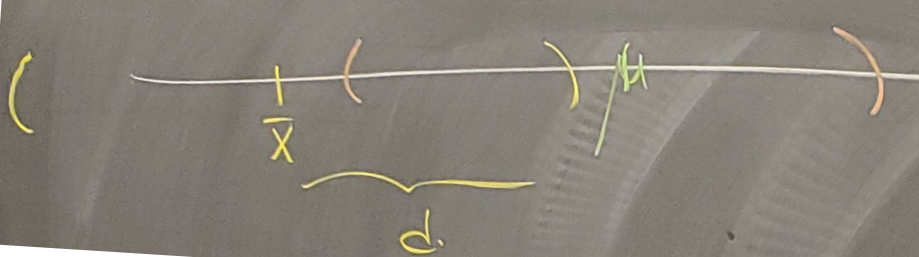
\includegraphics[width=5in]{10_3.png}\end{center}

\section{More about errors and sample size}

\nl \textbf{\color{eblue}Motivational example: } $X$ equals the breaking strength of a steel bar. If the bar is manufactured by Process I, it is known $X \sim N(50,\;36).$

\nl We now have Process II and it is hoped that the steel is 10\% stronger. i.e. $X \sim N(55,\;36)$.

\nl Our test? $$H_0 : \mu_I = 50 \hspace{1in} H_a : \mu_{II} = 55$$
{\red{Okay... we can't really test \say{this}}}

\nl But we can construct a hypothetical test where if $H_a$ is true, we can minimize (or control) both the Type I and Type II errors.

\nl For the sake of concrete-ness, set $n=16$. Then,
$$\sigma_{\Xbar}^2 = \frac{36}{16} \wideand \sigma_{\Xbar} = 1.5$$
\begin{center}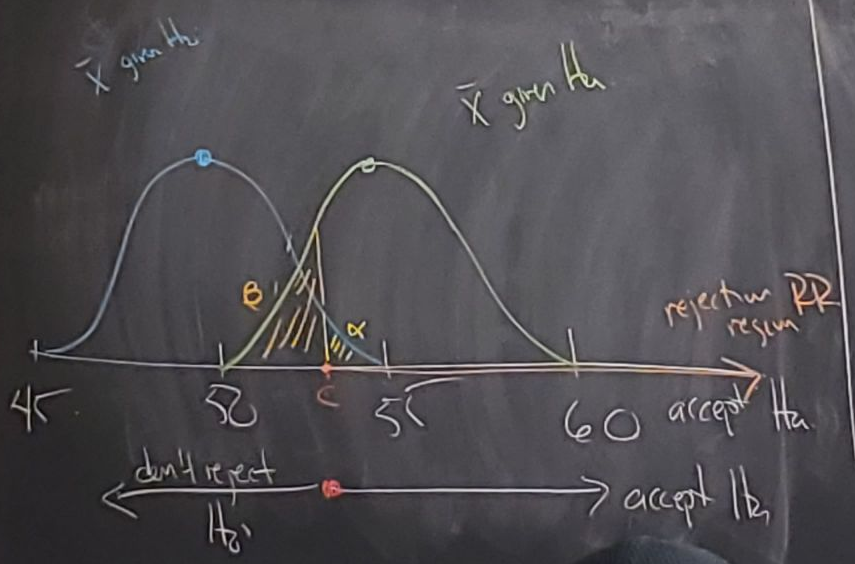
\includegraphics[width=6.5in]{2_25_1.png}\end{center}
$$\alpha = \P{\text{Type I}} \qquad H_0 : \mu = 50 \qquad H_a : \mu < 50$$
On the other hand, given $\alpha$, we can also see
$$\beta = \P{\text{Type II}} = \P{\text{accept } H_0 \text{ when } H_a \text{ is true}}$$


\nl Given $\alpha$, we can find $c$.
\begin{align*}
    \alpha &= \P{\Xbar > C \mid H_0}\\
    &= \P{\frac{\Xbar -{\color{blue}50}}{1.5} > \frac{C-{\color{blue}50}}{1.5}}
\end{align*}
and
\begin{align*}
    \beta &= \P{\Xbar < C \mid H_a}\\
    &= \P{\frac{\Xbar - {\color{ggreen}55}}{1.5} < \frac{C-{\color{ggreen}55}}{1.5}} 
\end{align*}
For fixed $n=16$, usually choose $\alpha$ small.
$$\alpha = \P{\Xbar -50 > 2\sigma_{\Xbar}} = 0.025$$%probably should be 1.960 instead of 2
Then $C = 50 + 2(1.5) = 53$ and
\begin{align*}
    \beta &= \P{\Xbar < 53 \mid H_a}\\
    &= \P{\frac{\Xbar - 55}{1.5} < 1.33}\\
    &= 0.0918
\end{align*}
Note almost four times as likely to make a Type II error than a Type I error. Of course, decreasing $\alpha$ with increase $\beta$.
$$\alpha = 0.01 \quad \implies \quad Z\text{-score} = 2.33 \qquad (Z_{0.98})$$
$$c = 50 + 2.33 (1.5) = 53.495$$
\begin{align*}
    \beta &= \P{\Xbar < 53.495 \mid H_a}\\
    &= \P{Z < -1.003}\\
    &= 0.1587
\end{align*}
Again, we note that the only way to decrease \textit{both} $\alpha$ and $\beta$ is to crank up the $n$.

\disc Choosing sample size $n$. We consider the 1-sided test
$$H_0 : \mu = \mu_0 \hspace{1in} H_a : \mu > \mu_0$$
Fix $\alpha$ at the start.
\begin{align*}
    \alpha &= \P{\Xbar > C \text{ when } \mu = \mu_0}\\
    &= \P{Z > \frac{C-\mu_0}{\sigma / \sqrt{n}}}\\
    &= \P{Z > Z_{\alpha}} \qquad Z_{\alpha} = \frac{C-\mu_0}{\sigma/\sqrt{n}}
\end{align*}
But, as with the power function, we need to choose specific $\mu_a$'s to work with (e.g. $\mu_a = 55$).
\begin{align*}
    \beta &= \P{\Xbar < C \text{ when } \mu = \mu_a}\\
    &= \P{Z < \frac{C-\mu_a}{\sigma / \sqrt{n}}}\\%
    &= \P{Z < -Z_{\beta}} \quad \text{when}\quad -Z_{\beta} = \frac{C-\mu_{\alpha}}{\sigma/\sqrt{n}}
\end{align*}
2 equations in the 2 unknows, $C,\;n$
$$C = \mu_0 + Z_{\alpha} \frac{\sigma}{\sqrt{n}} \wideand C = \mu_a - Z_{\beta} \frac{\sigma}{\sqrt{n}}$$
$$\mu + Z_{\alpha} \frac{\sigma}{\sqrt{n}} = \mu_a - Z_{\beta} \frac{\sigma}{\sqrt{n}} $$
Solve for $n$: 
$$(Z_{\alpha} + Z_{\beta})\frac{\sigma}{\sqrt{n}} = \mu_a - \mu_0$$
$$n = \frac{(Z_{\alpha} + Z_{\beta})^2 \sigma^2}{(\mu_a-\mu_0)^2}$$
Remark:
\begin{enumerate}[label=\textcircled{\raisebox{-1pt}{\arabic*}}]
    \item Of course all of this the fudge factor that we don't really know $\mu_a$.
    \item If we did $H_0 : \mu_0 = \mu_a$ and $H_a : \mu_0 > \mu_a$ we get the same formula for $n$. \say{sample size estimator for a one-sided $\alpha$-level test}
\end{enumerate}

\example* Back to the steel example

\nl If we decided at the start that we want $\alpha = \beta = 0.05$, what $n$ should we choose?

\nl For $\alpha = 0.05 \implies Z_{\alpha} = Z_{0.05} = 1.645$. Similarly for $\beta$, we need $Z_{\beta} = 1.645.$
Into our formula,
$$n = \pars{\frac{1.645+1.645}{\color{ggreen}55 \color{black} - \color{blue}50 \color{black}}}^2 \cdot 36 = \lceil 15.5867 \rceil = 16$$
Since we made $\alpha = \beta$ here, $C$ is the midpoint $C = \dfrac{55+50}{2} = 52.5$.
\begin{center}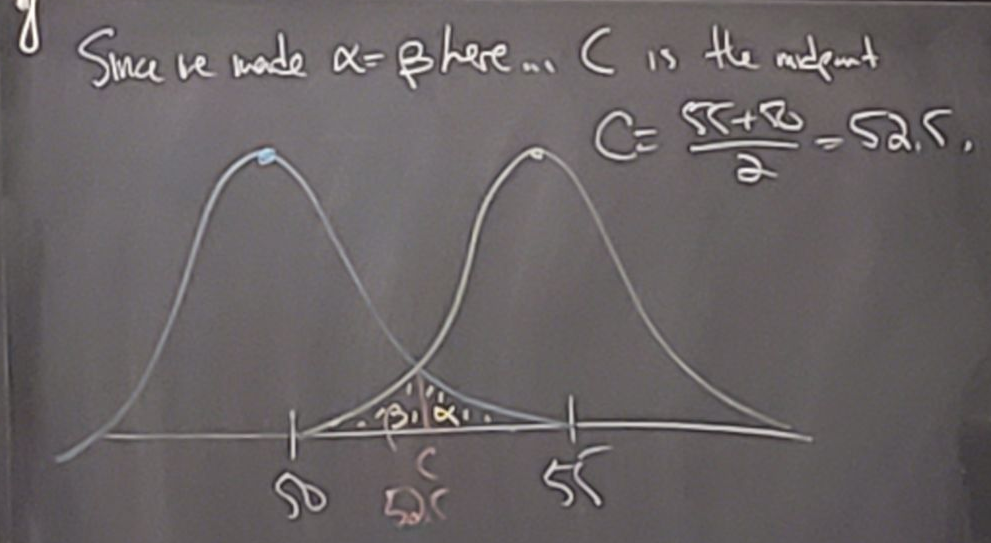
\includegraphics[width=4.5in]{2_25_2.png}\end{center}

\setSection{7}
\section{T tests} %10.8
Recall that for a small sample $n < 30$. We need to use the $t$-distribution.

\nl Chapter 8: t-stat confidence interval $\displaystyle \Xbar \pm t_{\alpha/2}(\text{df})\sqrt{\frac{s^2}{n}}$

\example 100 mL sample of water from swimming areas are tested for fecal colliform bacteria. It is considered to be safe if the level of bacteria is less than 400 in 3.3 oz.

\nl 20 Samples are taken: Found $\Xbar = 1231$ and $S = 1038$.

\nl Construct a test to determine if it's safe to swim. Our test:
\begin{align*}
    &H_0 : \mu_0 = 400\\
    &H_a : \mu_a > 400
\end{align*}
Test statistic $\displaystyle T = \frac{\Xbar - \mu_0}{S \big/ \sqrt{n}} = \frac{1231 - 1038}{1038\big/\sqrt{20}} = 0.350$ is the test statistic.

\nl The degrees of freedom is $n - 1 = 19$. Using table 5, $t_{0.005}(19)=2.861$ The $p$-value is: 
\begin{align*}
    p &= \Pr(T \geq 3.580 \mid \mu_0 = 400)\\
    &< \Pr(T \geq 2.861)\\
    &= 0.005
\end{align*}

\nl Reject $H_0$: There is poop in the water; stay out!

\remark* In general:
$$\displaystyle H_a := \begin{cases} \mu > \mu_0 \\ \setBlue \mu < \mu_0 \\ \setRed \mu \neq \mu_0 \end{cases} \implies \text{RR} := \underbrace{\begin{cases}t > t_{\alpha} \\ \setBlue t < -t_{\alpha}\\ \setRed \abs{t} > t_{\alpha/2} \end{cases}}_{\textstyle \text{the } t \text{-stat}}$$

\example Lifestyle comparison. Monitoring the active time (in minutes per day) between 2 populations: obese and lean.
\begin{center}
    \begin{tabular}{ |c|c|c|c| } 
        \hline
        \textbf{Group} & \textbf{Count} & \textbf{Standing/Walking} & $S$\\
        \hline
        Obese & $n=10$ & 373.269 & 67.498\\ 
        \hline
        Lean & $n=13$ &  525.751 & 107.121\\ 
        \hline
      \end{tabular}
    \end{center}


\nl Question: Are these two groups significant significant? This is a \say{are population means different} question.
\begin{align*}
    H_0 &: \mu_L = \mu_0 \quad \implies \quad  \mu_L - \mu_0 = 0\\
    H_a &: \mu_L \neq \mu_0 \quad \implies \quad \mu_L - \mu_0 \neq 0
\end{align*}
Questions about \say{\setRed different} results in a 2-sided test

\nl Confidence interval: $\displaystyle \Xbar_1 - \Xbar_2 \pm t_{\alpha/2}(\df)\pars{S_p\sqrt{\dfrac{1}{n_1} + \dfrac{1}{n_2}}}$
$$\color{orange} S_{\text{pool}} \setBlack = \sqrt{\dfrac{(n_1-1){S_1}^2 + (n_2-1){S_2}^2}{n_1 + n_2 - 2}} \quad \text{with } \df = n_1 + n_2 - 2$$
The difference in means $t$ test statistic is 
$$T = \dfrac{\Xbar_1 - \Xbar_2 - (\mu_1 - \mu_2)}{S_p \sqrt{\over*{n_1} + \over*{n_2}}}$$
Our $\Xbar_L - \Xbar_0 = 152.482$. $H_0 : \mu_L - \mu_0 = 0$ is the null hypothesis. $\df = 10+13-2=21.$
\begin{align*}
    S_p &= \sqrt{\dfrac{(13-1)107.121^2 + (10-1)67.498^2 }{13+10-2}}\\
    &= 92.247.\\
    \\
    T &= \frac{152.481}{92.247 \sqrt{\over*{10} + \over*{13}}}\\
    &= 3.93
    \\\\p &= \P{|T|>3.93} \\ &= 2 \cdot \P{T > 3.93}\\ &< 2 \cdot 0.0005 \tag{by table 5}\\
    & = 0.001
\end{align*}
So $p$ is super small ($p < \alpha$) which implies that we reject the null hypothesis. That is, $\mu_0 < \mu_L$ is true.

\nnl Our goal this week is to justify hypothesis testing. 

\nl Last day: Pearson Neyman Lamma

\nl $\thru{X} \sim$ via PDF $f(x \mid \theta)$ when $\theta_0$ and $\theta_a$ are two possible values of $\theta$. If there exists $a$ the constant $k$ and a subset $C$ of the sample space such that
\begin{enumerate}
    \item $P\{(\thru{x}) \in C \mid \theta_0\} = \alpha$
    \item $\dfrac{L(\theta_0)}{L(\theta_a)} \leq k$ for $\thru{x} \in C$.
    \item $\dfrac{L(\theta_0)}{L(\theta_a)} \geq k$ for $\thru{x} \in \overline{C}$
\end{enumerate}
Then $C$ is a best critical region of size $\alpha$ for testing $H_0 : \theta = \theta_0$ versus $H_a : \theta = \theta_a$.

\nl Before the proof\dots example.

\example Let $\thru{Y}$ from $\displaystyle f(y \mid \theta) = \frac{2}{\theta}y e^{-y^2/\theta}$ and $y > 0$. The Rayleight distribution.

\nl Want to test  $H_0 : \theta = \theta_0$ versus $H_a : \theta = \theta_a$.

\nl Note $\displaystyle L(\thru{Y} \mid \theta) = \frac{2}{\theta} y_i e^{-y_i^2/\theta} \cdots \frac{2}{\theta} y_n e^{-y_n^2/\theta}$.
$$\pars{\frac{2}{\theta}}^n \underbrace{\exp \brac{- \pars{\sum_1^n y_i^2} \bigg/ \theta }}_{g(S,\theta)} \underbrace{\prod_1^n y_i}_{h}$$
We will come back to this and connect to sufficiency next day.

The N-P ratio of likelihood function becomes
\begin{align*}
    \dfrac{L(\theta_0)}{L(\theta_a)} &= 
    \frac
    {\pars{\frac{2}{\theta_0}}^n \exp \brac{- \pars{\sum_1^n y_i^2} \bigg/ \theta_0 }\prod_1^n y_i}
    {\pars{\frac{2}{\theta_a}}^n \exp \brac{- \pars{\sum_1^n y_i^2} \bigg/ \theta_a }\prod_1^n y_i}\\
    &= \pars{\frac{\theta_a}{\theta_0}}^n \exp \brac{-\sum y_i^2 \cdot \pars{\over{\theta_0} - \over{\theta_a}}}
\end{align*}
We want $C$ to relate to our rejection region RR.

\nl So (2), implies \say{reject $H_0$ if}
$$\pars{\frac{\theta_a}{\theta_0}}^n \exp \brac{-\sum y_i^2 \cdot \pars{\over{\theta_0} - \over{\theta_a}}} \leq k$$
This looks scary, but $\theta_a$ and $\theta_0$ are fixed and $\theta_0 < \theta_a$ so $\pars{\over{\theta_0} - \over{\theta_a}} > 0$. In the end, making $\dfrac{L(\theta_0)}{L(\theta_a)}$ \say{small enough} for $k$ simlifies does to the condition that $\sum_{i}^n y_i^2$ is large enough. i.e. we need $\sum_1^n y_i^2 > k'$ for some $k'$ (dependent upon $k$). 

\nl New problem: To determine an appropriate $k'$, we need to know how $S = \sum_1^n y_i^2$ is distributed. 

\nl Using CDF method ($\S$ 6.3) we can show that the distribution of $y^2$ is exponention with mean $\theta$. Then, via products of moment generating functions. $$S = \sum_1^n y_i^2 \sim \operatorname{Gamma}\pars{n, \over{\theta}}$$
Stop! What just happened. 

\nl The N-P lemma tells us that the most powerful test of $H_0$ vs $H_a$ is to use the statistic $S = \sum y_i^2$. Then, given any $\alpha$ level significance (5\%, 1\%, whatever), we use the test on $S$ to be if $S$ is larger than $100(1-\alpha)$ percentile of the $\operatorname{Gamma}\pars{n, \over{\theta}}$ distribution\dots we reject $H_0$. 

\nl Picture with some $\gamma_*$ such that $\int_{\gamma_*}^{\infty} = \alpha$.

\nl $S > \gamma_*$, we reject the null hypothesis. Moreover, by the NP lemme, we don't have to compare the powe rof other possible tests because the lemma says any data
$$(\thru{Y}) \in C \leftrightsquigarrow S \geq \gamma_*$$
$$C := \left\{ (\thru{Y}) \mid \sum y_i^2 \geq \gamma_* \right\}$$
which is itself a consequence of our significance level $\alpha$ results in the most powerful test. 
$$P(C \mid \theta_a) \geq P(D \mid \theta_a)$$
where $D$ is another critical region $(P(D \mid \theta_a) = \alpha )$.

\defn The test using the best critical region is called the most powerful test. 

\nl Recap: We wanted to construct a hypothesis test at $\alpha$ significance level. All in one fell swoop, the N-P lemme says
\begin{enumerate}
    \item Here is the stat to use ($S = \sum y_i^2$ in last example) 
    \item Here is your rejection region ($S \geq \gamma_a$ in last example)
    \item in fact, this is the most powerful test possible.
\end{enumerate}
(This is kinda awesome)

Theorem: NP lemma;
\begin{proof} (Continuous)\\
    Let $B \subseteq \R^n$ and define $\displaystyle \underbrace{\int_B L(\theta) = \int \cdots \int}_{n \text{times}} L(\thru{x} \mid \theta) \, dx_1\, dx_2, \dots, dx_n  $.\\
    Assume there exists a critical region $C$ satisfying bullets 1 2 and 3.

    \nl $\alpha$ fixed, $\alpha = \int_C L(\theta_0)$ (same as $P(C \mid \theta_0)$)

    \nl Need to prove \say{best}, i.e. $P(C \mid \theta_a) \geq P(D \mid \theta_a)$

    \nl Assume $D$ is another critical region,
    $$\alpha = \int_D L(\theta)_0 = P(D\mid \theta_0)$$
    So $\displaystyle 0 = \int_C L(\theta_0) - \int_D L(\theta_0) $
    \begin{align*}0 &= \int_{C \cap D^C} L(\theta_0) + \int_{C \cap D} L(\theta_0) - \brac{ \int_{C \cap D} L(\theta_0) + \int_{C^C \cap D} L(\theta_0) }\\
        &= \int_{C \cap D^C} L(\theta_0) - \int_{C^C \cap D} L(\theta_0)\\
    &\text{By (2), there exists $k$ such that $\dfrac{L(\theta_0)}{L(\theta_a)} \leq k$ i.e. $L(\theta_0) \leq kL(\theta_a)$ at every point in $C$.}\\
    & \leq k \int_{C \cap D^C} L(\theta_a) - \int_{C^C \cap D} L(\theta_0)\\
    &\text{By (3) there exists $k$ such that $\dfrac{L(\theta_0)}{L(\theta_a)} \geq k$ i.e.  $L(\theta_0) \geq kL(\theta_a)$}\\
    & \leq k \brac{\int_{C \cap D^C} L(\theta_a) - \int_{C^C \cap D} L(\theta_a)}\\
    &= k \brac{\int_{C \cap D^C} L(\theta_a) + \int_{C \cap D} L(\theta_a) - \brac{ \int_{C \cap D} L(\theta_a) + \int_{C^C \cap D} L(\theta_a) }}\\
    &= k \brac{\int_C L(\theta_a) - \int_D L(\theta_a)}\\
    & \implies \int_C L(\theta_a) - \int_D L(\theta_a) \geq 0\\
    & \implies \int_C L(\theta_a) \geq \int_D L(\theta_a)\\
    & \implies P(C \mid \theta_a) \geq P(D \mid \theta_a)
    \end{align*}
    Here, $C$ is a best critical region of size $\alpha$ by defininition.
\end{proof}
\example Back to our old sample size example. 
$$\thru{X} \sim \operatorname{N}(\mu,\,36)$$
We played with $H_0 : \mu = 50$ and $H_a : \mu = 55$. 

\nl Consider the ratio of the likelihood functions.

\begin{align*}
    \frac{L(50)}{L(55)}
    &= \dfrac{(72 \pi)^{-n/2} \exp \brac{-\pars{\over{72}} \sum_1^n (X_i - 50)^2} }{{(72 \pi)^{-n/2} \exp \brac{-\pars{\over{72}} \sum_1^n (X_i - 55)^2} }}\\
    &= \exp \brac{ - \over{72} \sum_1^n \brac{(X_i-50)^2-(X_i-55)^2}}\\
    &= \exp \brac{-\over{72} \sum_1^n (10X_i -525) }\\
    &= \exp \brac{-\frac{5}{36} \sum_1^n X_i + \frac{175n}{24}} \leq k \text{ to satisfy (2)}\\
    & \implies -\frac{5}{36} \sum_1^n X_i + \frac{175n}{24} \leq \ln k\\
    & \implies \sum_1^n X_i \geq \frac{105n}
    {2} - \frac{36}{5} \ln k
    \\ & \implies \Xbar = \over{n}\sum_1^n X_i \geq \frac{105}{2} - \frac{36\ln k}{5n}
\end{align*}
We have our stat $\Xbar \geq k'$ thus will define our rejectoin rejection.

    %\text{    By (2), there exists $k$ such that $\dfrac{L(\theta_0)}{L(\theta_a)} \leq k$ i.e. $L(\theta_0) \leq kL(\theta_a)$ at every point in $C$.

    %By (3) there exists $k$ such that $\dfrac{L(\theta_0)}{L(\theta_a)} \geq k$ i.e.  $L(\theta_0) \geq kL(\theta_a)$}




% ^  stuff to finish








